% INTRODUÇÃO-------------------------------------------------------------------

\chapter{INTRODUÇÃO}
\label{chap:introducao}

\LaTeX{} é um conjunto de macros de alto nível para \TeX \xspace que torna mais fácil e rápida a produção de todo o tipo de documentos como, por exemplo, livros, relatórios e artigos.

O objetivo do \LaTeX \xspace é que o autor se possa distanciar da apresentação visual do trabalho e assim se concentrar no seu conteúdo. Possui formas de lidar com bibliografias, citações, formatos de páginas, referências e tudo mais que não seja relacionado com conteúdo do documento em si.

\section{Histórico}
\label{sec:Histórico}

Em 1978 Donald E. Knuth começou a desenvolver uma linguagem cujo objetivo era permitir a qualquer um formatar textos com muitas equações e com alta qualidade de saída, chamada de \TeX. Em 1985 Leisle Lamport desenvolveu um conjunto de macros denominado \LaTeX \xspace, que simplifica o uso da linguagem \TeX \xspace. Atualmente este projeto é mantido e desenvolvido pelo \LaTeX3 \xspace Project

O som final dos nomes \TeX \xspace e \LaTeX \xspace deve ser pronunciado como se fosse um “K”.

\section{Instalação}
\label{sec:Instalação}

\LaTeX é um software livre e gratuito, é possível instalar nos  principais sistemas operacionais modernos como: Windows 7, 8, 8.1 e 10; Mac OS e várias distribuições Linux.

\subsection{Windows}

MiKTeX é uma distribuição TeX / LaTeX para o Microsoft Windows. Baixe o instalador pelo link oficial: \href{https://miktex.org/download}{\textcolor{blue}{Download MiKTeX}}

A instalação do MiKTeX é simples, basicamente é só clicar no “Avançar”. Caso houver problemas na instalação o seguinte vídeo poderá servir de ajuda: \href{https://www.youtube.com/watch?v=4udFXbqtayE&list=LLQVoeslEpxQJ0UavpXUEkq}{\textcolor{blue}{Vídeo Instalação MiKTeX}}. Junto com a instalação do MiKTeX o editor TeXworks é instalado. Existem outros editores como o Texmaker. 

O Texmaker é mais simples de usar e é o editor de código aberto mais popular entre a comunidade LaTeX. Baixe o instalador pelo link oficial: \href{http://www.xm1math.net/texmaker/download.html}{\textcolor{blue}{Download TeXMaker}}

\subsection{Ubuntu}

O TeX Live é uma distribuição para produção de documentos \TeX \xspace. Para instalar no ubuntu 16.04 digite o seguinte comando: 
\begin{lstlisting}[language=bash]
    $ sudo apt-get install texlive-full
\end{lstlisting}

Apos a instalação do TeX Live pode-se obtar por instalar um editor específico para LaTeX o Texmaker, para instalar digite o seguinte comando: 

\begin{lstlisting}[language=bash]
    $ sudo apt-get install texmaker
\end{lstlisting}

\section{Compilação Tex Maker}

Para Compilar o arquivo \emph{.tex} junto com o arquivo \emph{.bib} no TeX Maker é necessário uma configuração, como mostra as Figuras \ref{fig:texmaker-config1} e \ref{fig:texmaker-config2}.

\begin{figure}[H]
    \centering
    \caption{Configuração Tex Maker}
    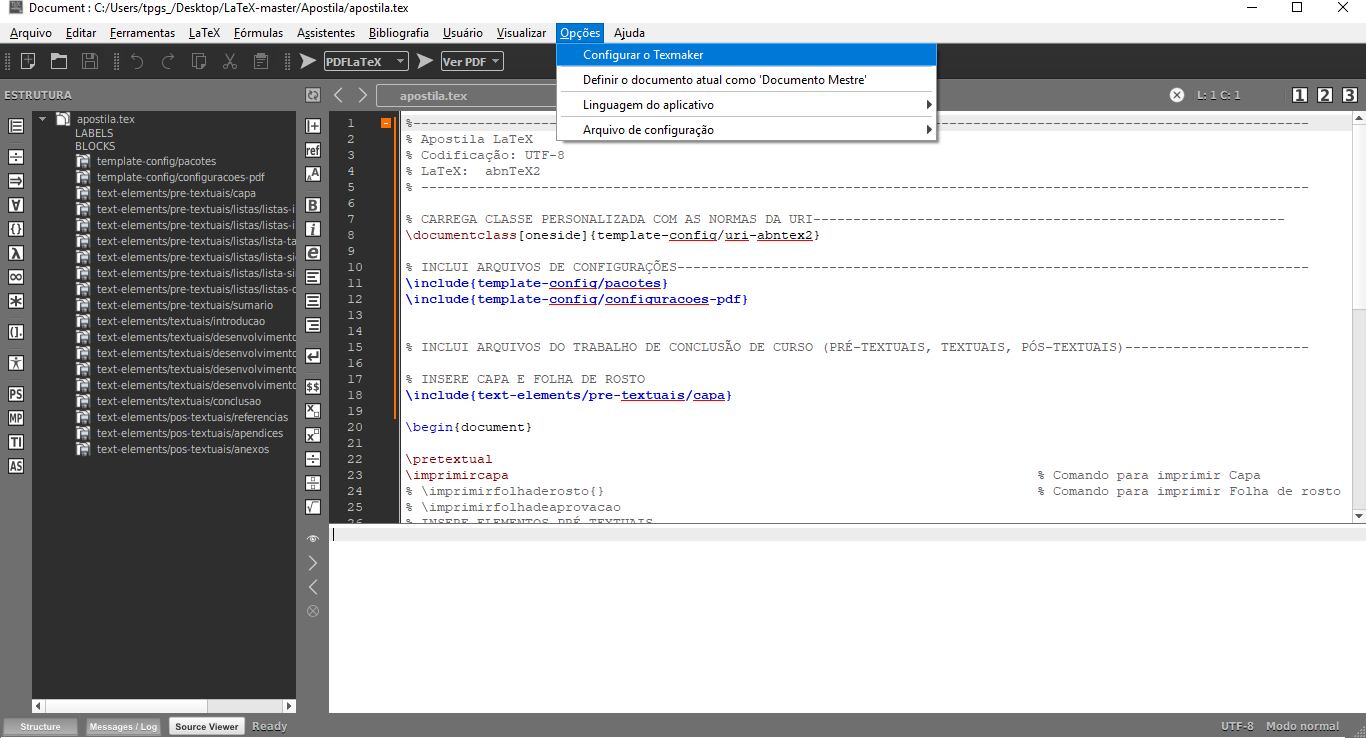
\includegraphics[width=0.70\textwidth]{./dados/figuras/compiler1}
    \fonte{Autor}
    \label{fig:texmaker-config1}
\end{figure}

\begin{figure}[H]
    \centering
    \caption{Configuração Tex Maker 2}
    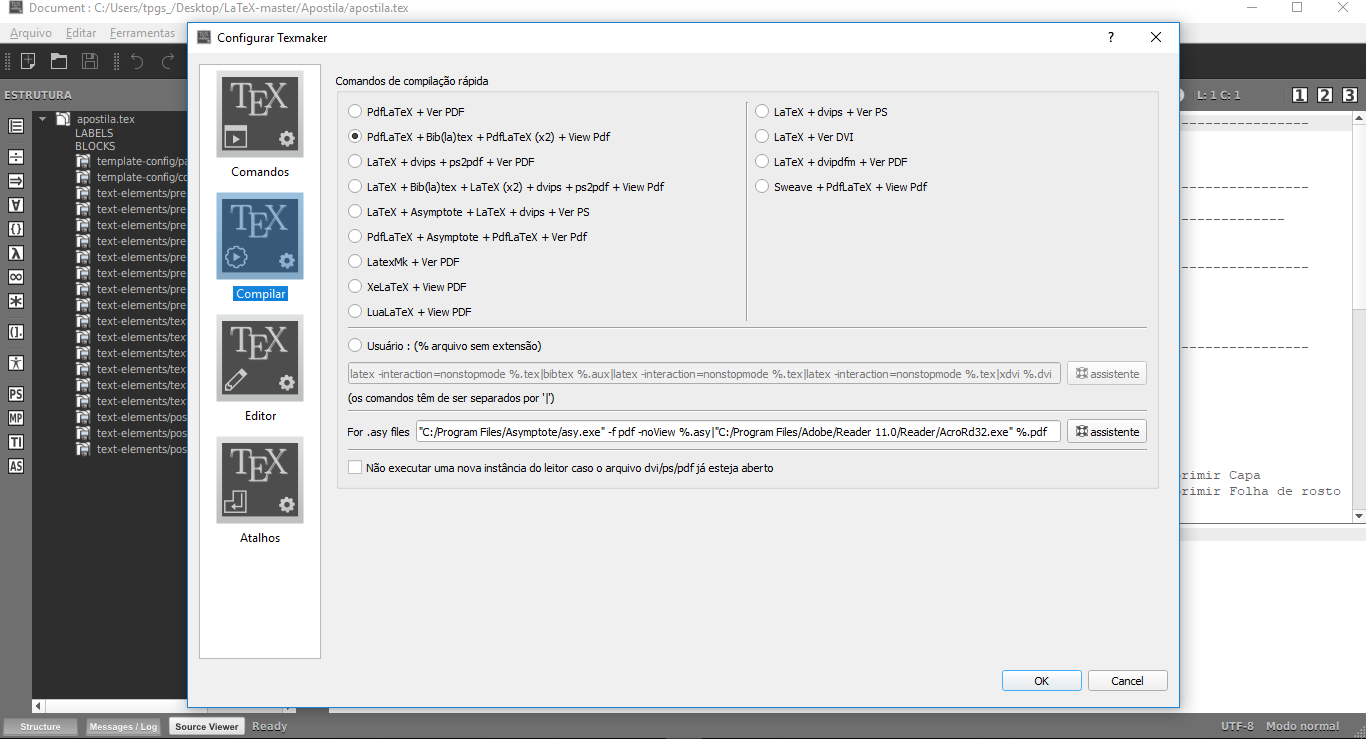
\includegraphics[width=0.70\textwidth]{./dados/figuras/compiler2}
    \fonte{Autor}
    \label{fig:texmaker-config2}
\end{figure}

\section{Compilação por Linha de Comando}

Para compilar pela linha de comando (windows e Linux) deve-se fazer os seguintes passos:

\begin{enumerate}
    \item Compilar o arquivo principal \emph{.tex}:
    \begin{lstlisting}[language=bash]
        pdflatex apostila.tex
    \end{lstlisting}
    \item Montar os índices:
    \begin{lstlisting}[language=bash]
        makeindex apostila.idx
    \end{lstlisting}
    \item Compilar o arquivo das bibliografias \emph{.bib}
    \begin{lstlisting}[language=bash]
        bibtex apostila.aux
    \end{lstlisting}
    \item Por fim, gerar o PDF:
    \begin{lstlisting}[language=bash]
        pdflatex apostila.tex
    \end{lstlisting}
\end{enumerate}

\section{Ferramentas em Nuvem}

Existem ferramentas que possibilitam a edição e a colaboração online de documentos LaTeX. Uma dessas ferramentas é o \href{https://www.overleaf.com/}{\textcolor{blue}{Overleaf}}.

Para usar o Overleaf basta criar uma conta, começar um projeto e escrever. Uma outra grande vantagem do Overleaf é a comunidade que compartilha templates prontos, como por exemplo:  \href{https://www.overleaf.com/latex/templates}{\textcolor{blue}{principais templates}}. 